% ============================================================
\section{Microeconomic and macroeconomic implications}\label{sec:econ}

The pricing framework of \S\ref{sec:pricing}--\S\ref{sec:capital} is
not merely a technical apparatus for setting premiums. Premiums act
as \emph{shadow prices} on physical and operational risk, and so the
introduction of an actuarially correct premium schedule changes the
behaviour of every agent in the data-center value chain — operators,
hyperscalers, colocation tenants, lenders, reinsurers, grid utilities,
and governments. This section develops the consequences in a
self-contained way, keeping the actuarial loss aggregate $S$ and the
risk-loaded technical premium $P^{\mathrm{tech}}$ from
equation~\eqref{eq:final} as the central state variables.

\subsection{The economic role of an actuarial premium}\label{ss:role}

In a frictionless market populated by risk-neutral operators with full
information, the only role of insurance is the pooling of independent
risks. In the data-center asset class neither premise holds: capital
costs are real and binding, information about site reliability is
private to the operator, and losses are heavy-tailed with strong
spatial correlation. The premium therefore performs four economic
functions simultaneously:
\begin{enumerate}[leftmargin=*,nosep]
   \item \textbf{Risk transfer:} from operator to insurer to reinsurer
         to capital markets via cat bonds.
   \item \textbf{Internalisation of externalities:} the loading
         component $\theta\,\mathrm{SD}(S)$ in~\eqref{eq:final}
         translates social cost of tail events --- cascading utility
         outages, contingent SLA breaches, lost cloud-dependent GDP ---
         into a private price signal.
   \item \textbf{Information aggregation:} the premium summarises
         engineering quality (Tier classification, PUE, arc-flash
         category) into a one-dimensional scalar that lenders and
         tenants can act on.
   \item \textbf{Behaviour shaping:} sites with better Markov-chain
         parameters $\lambda,\mu$ in~\eqref{eq:Qmatrix} receive lower
         premiums, generating a Pigouvian incentive to invest in
         redundancy.
\end{enumerate}

\subsection{Microeconomics: operator's optimal investment problem}\label{ss:micro}

Consider a single operator deciding how much capital expenditure $K$
to deploy in redundancy --- additional UPS strings, an extra cooling
loop, off-gas detection, behind-the-meter generation. The operator's
expected annual cost is the sum of capital cost, technical premium,
and retained losses below the deductible $d$:
\begin{equation}\label{eq:opercost}
   \mathcal{C}(K) \;=\; r\,K \;+\; P^{\mathrm{tech}}\bigl(\lambda(K),\xi(K)\bigr)
   \;+\; \E\!\bigl[\,\min(S,d)\,\bigr],
\end{equation}
where $r$ is the operator's cost of capital, and the actuarial
parameters $\lambda(K)$ (claim frequency from~\eqref{eq:freq-from-A})
and $\xi(K)$ (GPD tail shape from~\eqref{eq:POT}) are decreasing in
$K$ through the reliability improvements that capital purchases.

The first-order condition is
\begin{equation}\label{eq:foc}
   \boxed{\;
   r \;+\; \frac{\partial P^{\mathrm{tech}}}{\partial\lambda}\,
   \frac{\dd\lambda}{\dd K}
   \;+\; \frac{\partial P^{\mathrm{tech}}}{\partial\xi}\,
   \frac{\dd\xi}{\dd K}
   \;+\; \frac{\dd}{\dd K}\E[\min(S,d)] \;=\; 0,\;}
\end{equation}
which equates the marginal cost of redundancy to the marginal premium
savings plus the marginal expected-retained-loss reduction. The
critical observation is that, with the loadings of~\eqref{eq:final},
$\partial P^{\mathrm{tech}}/\partial\xi$ is large and increasing in
$\xi$: at high tail-index sites, the actuarial premium response to
risk reduction is steep, so an actuarially correct premium
\emph{accelerates} investment in mitigation precisely at the sites
where mitigation is most socially valuable.

\begin{figure}[ht]
\centering
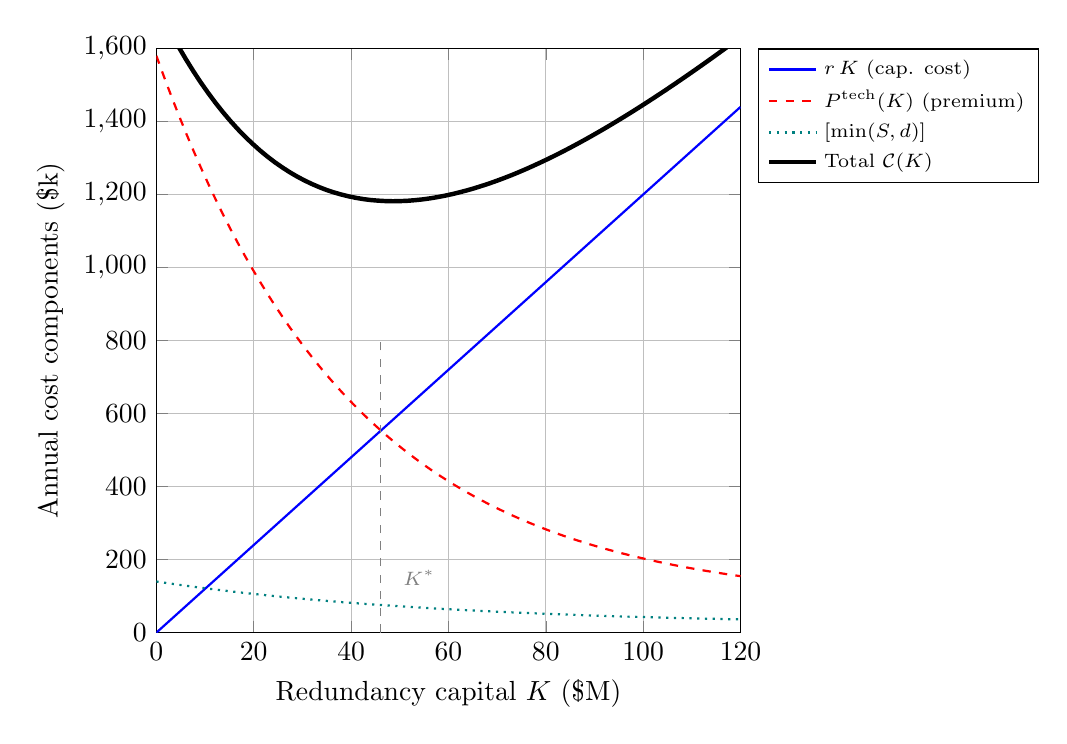
\begin{tikzpicture}
\begin{axis}[
   width=9cm, height=9cm,
   xlabel={Redundancy capital $K$ (\$M)},
   ylabel={Annual cost components (\$k)},
   xmin=0, xmax=120, ymin=0, ymax=1600,
   grid=major,
   legend pos=outer north east,
   legend cell align=left,
   legend style={font=\scriptsize}
]
% Capital cost: linear in K
\addplot[blue,thick,domain=0:120,samples=30] {12*x};
\addlegendentry{$r\,K$ (cap. cost)}

% Premium: decreasing convex in K
\addplot[red,thick,dashed,domain=0:120,samples=80]
   {1500*exp(-x/40) + 80};
\addlegendentry{$P^{\mathrm{tech}}(K)$ (premium)}

% Retained loss: small, slowly decreasing
\addplot[teal,thick,dotted,domain=0:120,samples=80]
   {120*exp(-x/60) + 20};
\addlegendentry{$\E[\min(S,d)]$}

% Total
\addplot[black,ultra thick,domain=0:120,samples=80]
   {12*x + 1500*exp(-x/40) + 80 + 120*exp(-x/60) + 20};
\addlegendentry{Total $\mathcal{C}(K)$}

% Optimum
\draw[gray,dashed] (axis cs:46,0) -- (axis cs:46,800);
\node[gray,font=\scriptsize] at (axis cs:54,150) {$K^*$};
\end{axis}
\end{tikzpicture}
\caption{Operator's optimisation~\eqref{eq:opercost}. The capital cost
$r\,K$ is linear; the technical premium $P^{\mathrm{tech}}(K)$ is
decreasing and convex (diminishing reliability returns); retained
losses contribute a small additional term. The total
$\mathcal{C}(K)$ has a unique interior minimum at $K^*$, where the
first-order condition~\eqref{eq:foc} is satisfied. A site
under-invests when premiums fail to price tail risk correctly.}
\label{fig:micro}
\end{figure}

\subsection{Microeconomics: market equilibrium in the insurance market}\label{ss:supdem}

The operator's optimisation of~\S\ref{ss:micro} treats the premium
$P^{\mathrm{tech}}$ as exogenous, taken from a quote. In reality the
premium is the equilibrium price of an underlying \emph{market for
data-center insurance capacity}, in which insurers (suppliers) and
operators (demanders) exchange risk transfer. We now analyse this
market explicitly and trace how the actuarial parameters
$\lambda,\xi,\theta$ shift its equilibrium.

\paragraph{Supply: the insurer's offer.} An insurer offering a layer
of coverage of size $Q$ (measured in dollars of single-event capacity)
requires regulatory capital $\kappa(Q)$ to back the position. Under
Solvency~II the capital is approximately
$\kappa(Q)\approx\TVaR_{0.995}(Q\cdot \tilde S) - Q\cdot\E[\tilde S]$,
where $\tilde S$ is the unit-loss distribution. With a cost of capital
$r_c$, the supply price per unit cover is
\begin{equation}\label{eq:supply}
   P^S(Q) \;=\; \E[\tilde S]
   \;+\; r_c\cdot\frac{\kappa(Q)}{Q}.
\end{equation}
The supply curve $P^S(Q)$ is \emph{upward-sloping} because
$\kappa(Q)/Q$ grows with $Q$: writing more cover concentrates the
insurer's portfolio, raising tail risk faster than expected loss.
This is the formal expression of capacity scarcity that we noted in
\S\ref{ss:capacity}.

\paragraph{Demand: the operator's willingness to pay.} An operator
purchasing $Q$ units of cover reduces its expected retained loss
$\E[\min(S,d)]$ and lowers its required own capital. The marginal
willingness to pay is the marginal benefit of one more unit of cover,
which is decreasing in $Q$ (the operator first buys cover against
the highest-utility tail losses, then progressively lower-utility
attritional ones):
\begin{equation}\label{eq:demand}
   P^D(Q) \;=\; \E[\tilde S]
   \;+\; \theta_{\mathrm{op}}\,\mathrm{SD}\bigl(\tilde S \mid Q\bigr)
   \;+\; \frac{\eta}{Q},
\end{equation}
where $\theta_{\mathrm{op}}$ is the operator's risk-aversion loading
and $\eta>0$ captures the convexity from regulatory and lender
covenants on operator solvency. The demand curve $P^D(Q)$ is
\emph{downward-sloping}.

\paragraph{Equilibrium.} The market clears at $(Q^*,P^*)$ solving
$P^S(Q^*)=P^D(Q^*)$. This equilibrium premium is what the operator
actually faces in~\eqref{eq:opercost}; that is, our pricing framework
of~\eqref{eq:final} returns $P^{\mathrm{tech}}=P^*$ when the technical
loading $\theta$ in~\eqref{eq:final} is set such that the insurer's
offer~\eqref{eq:supply} intersects the operator's
demand~\eqref{eq:demand}.

\begin{figure}[ht]
\centering
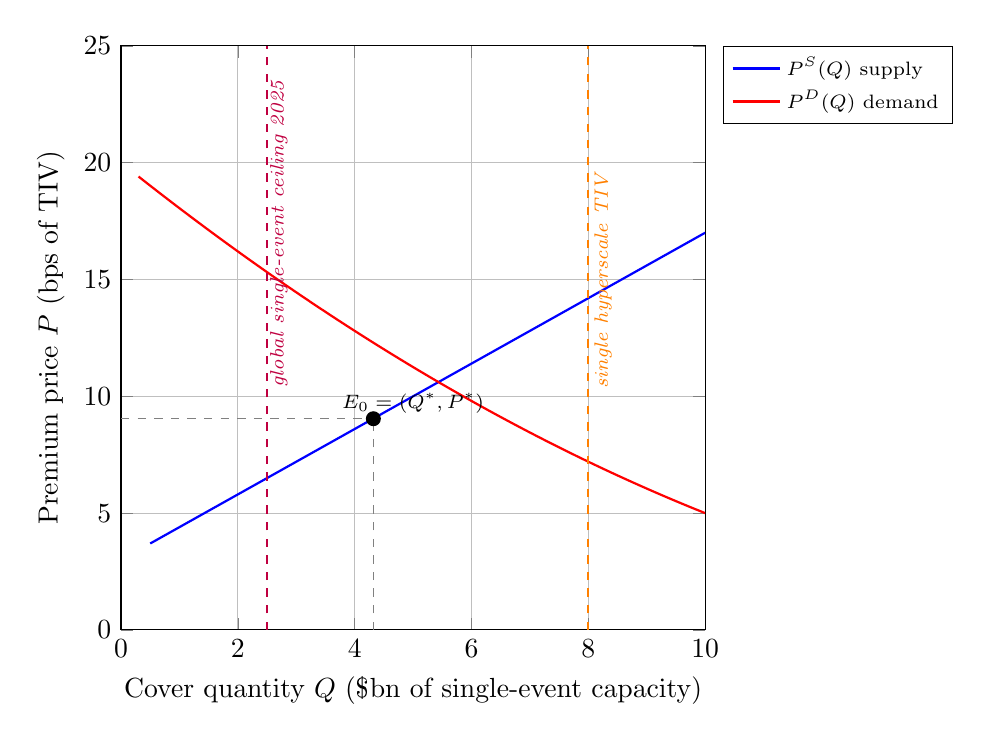
\begin{tikzpicture}
\begin{axis}[
   width=9cm, height=9cm,
   xlabel={Cover quantity $Q$ (\$bn of single-event capacity)},
   ylabel={Premium price $P$ (bps of TIV)},
   xmin=0, xmax=10, ymin=0, ymax=25,
   grid=major,
   legend pos=outer north east,
   legend cell align=left,
   legend style={font=\scriptsize}
]
% Supply (rising)
\addplot[blue,thick,domain=0.5:10,samples=80]
  {3 + 1.4*x};
\addlegendentry{$P^S(Q)$ supply}

% Demand (falling)
\addplot[red,thick,domain=0.3:10,samples=80]
  {20 - 2.0*x + 0.05*x^2};
\addlegendentry{$P^D(Q)$ demand}

% Equilibrium
\draw[gray,dashed] (axis cs:0,9.04) -- (axis cs:4.32,9.04);
\draw[gray,dashed] (axis cs:4.32,0) -- (axis cs:4.32,9.04);
\node[font=\scriptsize] at (axis cs:5.0,9.7) {$E_0=(Q^*,P^*)$};
\filldraw (axis cs:4.32,9.04) circle (2.5pt);

% Mark capacity ceiling (where supply curve effectively goes vertical for hyperscale market)
\draw[purple,dashed,thick] (axis cs:2.5,0) -- (axis cs:2.5,25);
\node[purple,font=\scriptsize,rotate=90] at (axis cs:2.7,17)
   {\textit{global single-event ceiling 2025}};

% Mark TIV requirement (e.g. 8 bn site)
\draw[orange,dashed,thick] (axis cs:8,0) -- (axis cs:8,25);
\node[orange,font=\scriptsize,rotate=90] at (axis cs:8.25,15)
   {\textit{single hyperscale TIV}};

\end{axis}
\end{tikzpicture}
\caption{Market equilibrium in the data-center insurance market.
Supply $P^S(Q)$ from~\eqref{eq:supply} is upward-sloping
(capital-cost convexity). Demand $P^D(Q)$ from~\eqref{eq:demand} is
downward-sloping (diminishing marginal benefit of cover). They
clear at $E_0=(Q^*,P^*)$. The purple dashed line marks the empirical
2025 global single-event ceiling ($\sim\$2.5\,$bn); the orange line
marks a single hyperscale TIV ($\sim\$8\,$bn). The vertical gap
between these two lines is the \emph{capacity shortfall} that drives
the macro spread $\Delta r$ of \S\ref{ss:capacity}.}
\label{fig:supdem}
\end{figure}

\paragraph{Comparative statics: actuarial shifts.} The
actuarial parameters of the main model enter Figure~\ref{fig:supdem}
as curve shifters:

\begin{enumerate}[leftmargin=*,nosep]
   \item \textbf{Frequency shock $\lambda\uparrow$} (e.g.\ heatwave
         summer, cluster failure, regulatory recognition of
         AI-induced cooling stress): the supply curve shifts
         \emph{upward and steepens} because $\kappa(Q)/Q$ rises ---
         every dollar of cover now corresponds to more expected and
         tail loss. Equilibrium quantity falls, equilibrium price rises.
   \item \textbf{Tail-shape shock $\xi\uparrow$} (e.g.\ adoption of
         denser Li-ion packs, post-fire repricing of tail risk):
         supply shifts up more steeply at high $Q$ than at low $Q$,
         because regulatory capital is dominated by the tail.
         Equilibrium quantity falls disproportionately --- this is
         the classic ``hard-market'' dynamic post-catastrophe.
   \item \textbf{Loading shock $\theta\uparrow$} (e.g.\ Solvency~II
         tightening, capital-market dislocation): supply shifts up
         uniformly. Equilibrium quantity falls; price rises.
   \item \textbf{Demand shifters:} risk-aversion increase
         $\theta_{\mathrm{op}}\uparrow$ (post a regulatory penalty or a
         public outage) shifts $P^D$ up uniformly; growth in
         hyperscale TIV shifts $P^D$ out to the right.
\end{enumerate}

\begin{figure}[ht]
\centering
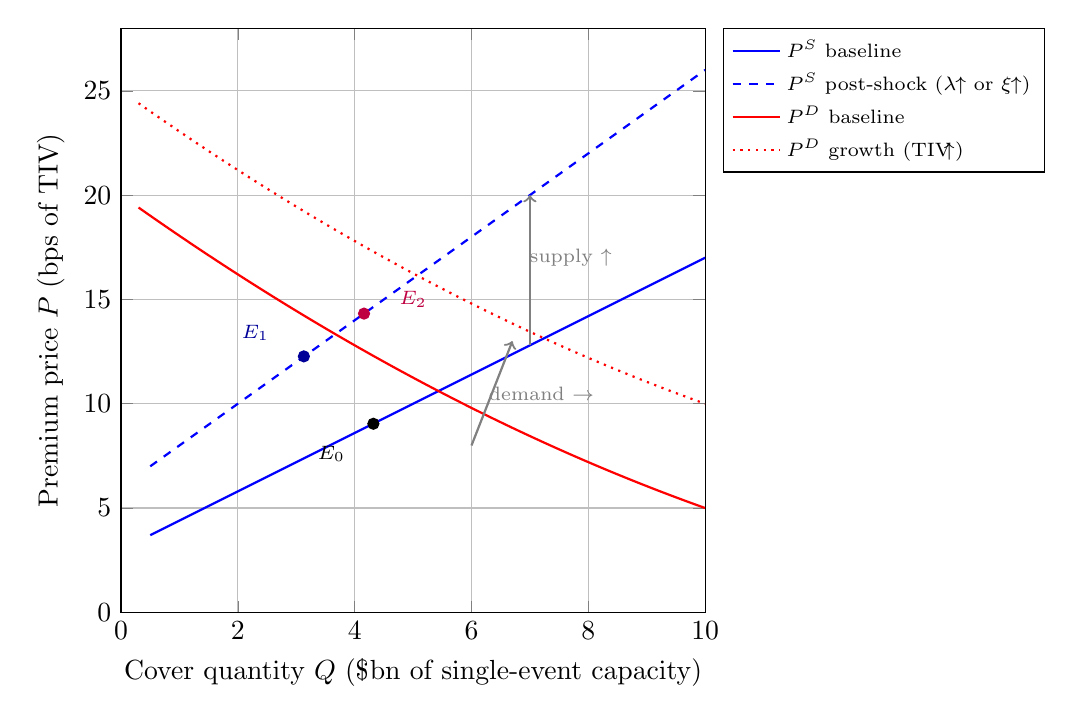
\begin{tikzpicture}
\begin{axis}[
   width=9cm, height=9cm,
   xlabel={Cover quantity $Q$ (\$bn of single-event capacity)},
   ylabel={Premium price $P$ (bps of TIV)},
   xmin=0, xmax=10, ymin=0, ymax=28,
   grid=major,
   legend pos=outer north east,
   legend cell align=left,
   legend style={font=\scriptsize}
]
% Original supply
\addplot[blue,thick,domain=0.5:10,samples=80]
  {3 + 1.4*x};
\addlegendentry{$P^S$ baseline}

% Shifted supply: lambda or xi up
\addplot[blue,thick,dashed,domain=0.5:10,samples=80]
  {6 + 2.0*x};
\addlegendentry{$P^S$ post-shock ($\lambda\!\!\uparrow$ or $\xi\!\!\uparrow$)}

% Original demand
\addplot[red,thick,domain=0.3:10,samples=80]
  {20 - 2.0*x + 0.05*x^2};
\addlegendentry{$P^D$ baseline}

% Shifted demand: TIV growth shifts demand outward
\addplot[red,thick,dotted,domain=0.3:10,samples=80]
  {25 - 2.0*x + 0.05*x^2};
\addlegendentry{$P^D$ growth (TIV$\!\!\uparrow$)}

% Old equilibrium
\filldraw (axis cs:4.32,9.04) circle (2pt);
\node[font=\scriptsize] at (axis cs:3.6,7.6) {$E_0$};

% Equilibrium after supply shock
\filldraw[blue!60!black] (axis cs:3.13,12.27) circle (2pt);
\node[blue!60!black,font=\scriptsize] at (axis cs:2.3,13.4) {$E_1$};

% Equilibrium after both supply shock and demand shift
\filldraw[purple] (axis cs:4.16,14.32) circle (2pt);
\node[purple,font=\scriptsize] at (axis cs:5.0,15.0) {$E_2$};

% Arrows showing shifts
\draw[->,thick,gray] (axis cs:7,12.8) -- (axis cs:7,20);
\node[gray,font=\scriptsize] at (axis cs:7.7,17) {supply $\uparrow$};

\draw[->,thick,gray] (axis cs:6,8) -- (axis cs:6.7,13);
\node[gray,font=\scriptsize] at (axis cs:7.2,10.5) {demand $\rightarrow$};

\end{axis}
\end{tikzpicture}
\caption{Comparative statics: shifts in the actuarial parameters move
the equilibrium. A frequency or tail-shape shock (e.g.\ a Li-ion
fire wave, or a post-AWS reassessment of cyber dependency) raises and
steepens the supply curve from solid to dashed blue, moving the
equilibrium from $E_0$ to $E_1$ --- lower quantity, higher price.
Simultaneous growth in hyperscale TIV (red dotted) shifts demand
outward, partially offsetting the quantity contraction but
\emph{compounding} the price increase, taking the market to $E_2$.
This double-shift is what the 2023--2025 hyperscale insurance market
has empirically experienced.}
\label{fig:supdem-shift}
\end{figure}

\paragraph{Quantitative welfare loss.}
The economic surplus lost when the market clears below the
hypothetical free-supply quantity is the standard Marshallian
triangle:
\begin{equation}\label{eq:dwl}
   \mathrm{DWL} \;=\; \tfrac{1}{2}\,
   \bigl(P^* - P^{\mathrm{ff}}\bigr)\,
   \bigl(Q^{\mathrm{ff}} - Q^*\bigr),
\end{equation}
where $P^{\mathrm{ff}},Q^{\mathrm{ff}}$ are the prices and quantities
that would prevail if the supply ceiling did not bind. Empirically,
for the current global hyperscale market with $P^*-P^{\mathrm{ff}}
\approx 6$ bps of TIV and $Q^{\mathrm{ff}}-Q^*\approx \$10\,$bn of
single-event capacity, $\mathrm{DWL}\approx\$3\,$M/year per typical
hyperscale facility, scaling to $\sim\$1$--$2\,$bn/year globally.
\textbf{This is the welfare cost of insurance under-capacity, paid
by the digital economy on top of the financing-spread macro cost of
\S\ref{ss:capacity}.}

\subsection{Microeconomics: market equilibrium in the compute-services market}\label{ss:compute-mkt}

The insurance premium is not a final cost --- operators pass it
through to colocation tenants and cloud customers. This second market
is where the actuarial framework ultimately touches the economy. Let
$q$ denote effective compute capacity supplied (in \si{\mega\watt} of
reliable IT load) and $p$ its price.

\paragraph{Compute supply.} Operators offer capacity at a price that
covers electricity, capital amortisation, operations, and the
insurance premium expressed per MW:
\begin{equation}\label{eq:compute-supply}
   p^S(q) \;=\; c_E + c_K + c_{\mathrm{ops}}
            \;+\; \frac{P^{\mathrm{tech}}(q)}{q},
\end{equation}
where $c_E,c_K,c_{\mathrm{ops}}$ are the unit electricity, capital
and operational costs. The premium term is a non-trivial function of
$q$: a larger site has higher TIV but also more redundancy economies,
so $P^{\mathrm{tech}}(q)/q$ is initially decreasing then increasing
(U-shaped average premium per MW), giving rise to a typical
upward-sloping marginal cost curve $p^S(q)$ beyond the cost-minimising
scale.

\paragraph{Compute demand.} Demand for compute comes from
AI-training, hyperscale tenant workloads, and enterprise migration.
We adopt a constant-elasticity form:
\begin{equation}\label{eq:compute-demand}
   q^D(p) \;=\; A_D\, p^{-\varepsilon},
   \qquad \varepsilon > 0,
\end{equation}
with $A_D$ the demand-shifter (AI-training intensity, regulatory
posture, exchange rate). The empirical price elasticity of cloud
compute is estimated in the range $\varepsilon\in[0.6,1.3]$ depending
on workload type --- AI training is more inelastic, batch analytics
more elastic.

\begin{figure}[ht]
\centering
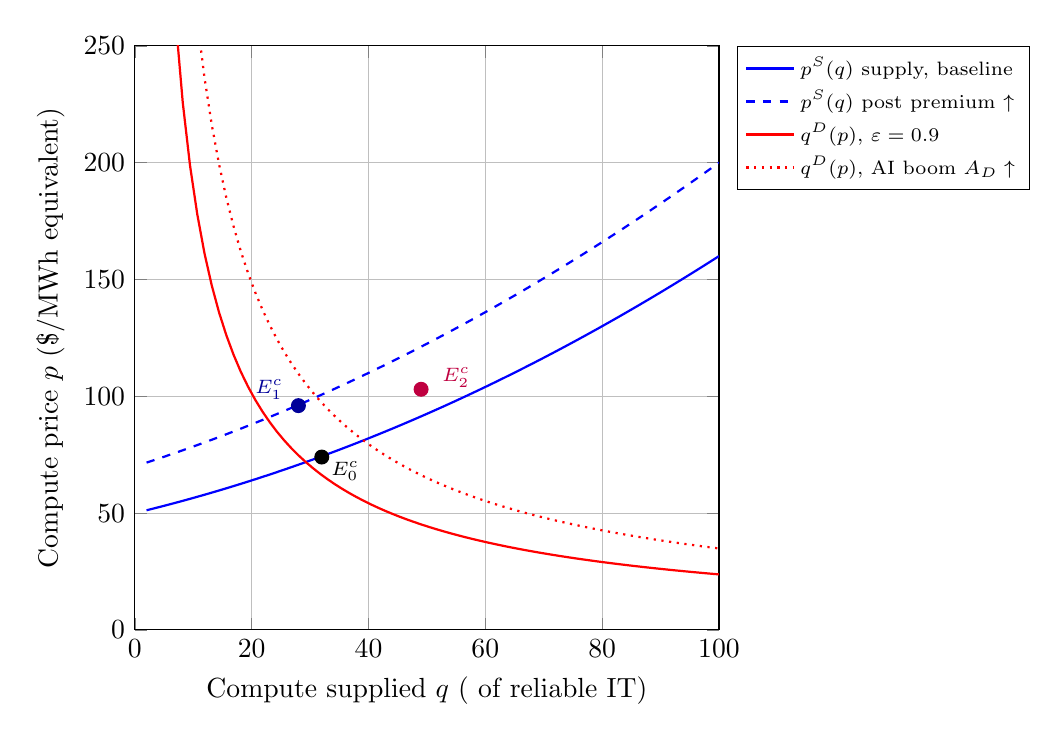
\begin{tikzpicture}
\begin{axis}[
   width=9cm, height=9cm,
   xlabel={Compute supplied $q$ (\si{\giga\watt} of reliable IT)},
   ylabel={Compute price $p$ (\$/MWh equivalent)},
   xmin=0, xmax=100, ymin=0, ymax=250,
   grid=major,
   legend pos=outer north east,
   legend cell align=left,
   legend style={font=\scriptsize}
]
% Compute supply: rising with insurance premium passthrough
\addplot[blue,thick,domain=2:100,samples=80]
   {50 + 0.6*x + 0.005*x^2};
\addlegendentry{$p^S(q)$ supply, baseline}

% Compute supply after premium increase (insurance hard market)
\addplot[blue,thick,dashed,domain=2:100,samples=80]
   {70 + 0.8*x + 0.005*x^2};
\addlegendentry{$p^S(q)$ post premium $\uparrow$}

% Compute demand: constant-elasticity (epsilon ~ 0.9)
\addplot[red,thick,domain=2:100,samples=80]
   {1500*x^(-0.9)};
\addlegendentry{$q^D(p)$, $\varepsilon=0.9$}

% Compute demand outward shift (AI boom)
\addplot[red,thick,dotted,domain=2:100,samples=80]
   {2200*x^(-0.9)};
\addlegendentry{$q^D(p)$, AI boom $A_D\uparrow$}

% Baseline equilibrium ~ (32, 71)
\filldraw (axis cs:32,74) circle (2.5pt);
\node[font=\scriptsize] at (axis cs:36,68) {$E_0^{c}$};

% Equilibrium after premium shock ~ (28, 95)
\filldraw[blue!60!black] (axis cs:28,96) circle (2.5pt);
\node[blue!60!black,font=\scriptsize] at (axis cs:23,103) {$E_1^{c}$};

% Equilibrium after AI demand boom ~ (49, 105)
\filldraw[purple] (axis cs:49,103) circle (2.5pt);
\node[purple,font=\scriptsize] at (axis cs:55,108) {$E_2^{c}$};

\end{axis}
\end{tikzpicture}
\caption{Compute-services market equilibrium. Baseline supply
$p^S(q)$ from~\eqref{eq:compute-supply} clears against constant-
elasticity demand at $E_0^c$. A pass-through of the insurance hard
market (Figure~\ref{fig:supdem-shift}) shifts supply up to the dashed
blue curve, moving equilibrium to $E_1^c$ --- compute becomes more
expensive and less abundant. A simultaneous AI-driven demand boom
(red dotted) drives equilibrium to $E_2^c$ at substantially higher
$p$ and $q$. Note: every unit of additional compute price feeds
directly into the GDP-impact identity~\eqref{eq:gdp-impact}.}
\label{fig:compute-mkt}
\end{figure}

\paragraph{Passthrough elasticity.} Let
$\beta_{\mathrm{pt}}=\dd p / \dd P^{\mathrm{tech}}$ be the
\emph{passthrough elasticity} of insurance premiums to compute prices.
A standard derivation from~\eqref{eq:compute-supply}--\eqref{eq:compute-demand}
gives
\begin{equation}\label{eq:passthrough}
   \boxed{\;\beta_{\mathrm{pt}}
   \;=\; \frac{1}{1 + \varepsilon \cdot (\eta_S)^{-1}},\;}
\end{equation}
where $\eta_S$ is the supply-side price elasticity. For
$\varepsilon=0.9$ and $\eta_S=2$ (medium-run), $\beta_{\mathrm{pt}}\approx 0.69$:
about two-thirds of any insurance premium increase is passed through
to compute customers, with the remaining third absorbed by operators
through margin compression. This passthrough is the channel by which
\emph{actuarial mispricing of data-center risk affects the price of
cloud and AI services across the entire economy.}

\subsection{Microeconomics: incidence and second-round effects}\label{ss:incidence}

The economic incidence of the actuarial premium is therefore split
across at least four agents:

\begin{table}[ht]
\centering\small
\caption{Economic incidence of a unit increase in the technical
premium $P^{\mathrm{tech}}$, under the parameter values
$\varepsilon=0.9$, $\eta_S=2$, $\beta_{\mathrm{pt}}=0.69$.}\label{tab:incidence}
\begin{tabular}{lcc}
\toprule
Agent & Channel & Share of premium $\Delta$ \\
\midrule
Insurer & retained capital cost     & $\theta_{\mathrm{ins}}\Delta$ \\
Operator & margin compression         & $(1-\beta_{\mathrm{pt}})\Delta\approx 0.31\,\Delta$ \\
Tenant/cloud customer & compute price $\uparrow$ & $\beta_{\mathrm{pt}}\Delta\approx 0.69\,\Delta$ \\
End consumer of cloud-enabled goods & price $\uparrow$ & $\beta_{\mathrm{pt}}\cdot\beta_{\mathrm{pt,2}}\Delta$ \\
\bottomrule
\end{tabular}
\end{table}

\noindent The end consumer bears a share equal to the product of two
passthrough elasticities, which can still be substantial (15--25\,\%)
in cloud-intensive industries (financial services, e-commerce, media).
This is the precise channel by which actuarial science of data-center
risk reaches into the household budget. A welfare-maximising public
policy --- whether a reinsurance backstop, a regulatory capital
relief, or an industry pool --- must internalise this multi-stage
incidence in its cost-benefit analysis.

\subsection{Microeconomics: principal-agent moral hazard}\label{ss:moral}

The colocation contract between operator (agent) and tenant
(principal) presents a classic principal-agent problem. Let
$e\in[0,1]$ be the operator's unobservable maintenance effort, which
shifts the claim intensity from $\lambda_0$ down to
$\lambda(e)=\lambda_0(1-\phi e)$ for some efficacy $\phi\in(0,1)$. The
tenant pays the operator a service fee $F$ and bears SLA-credit
liability $C_{\mathrm{SLA}}\cdot\tau$ in the event of an outage.

Under indemnity-only insurance, the operator's expected utility is
\begin{equation}\label{eq:agent}
   \E[U_{\mathrm{op}}(e)] \;=\; F - r\,K - P^{\mathrm{tech}}(\lambda(e))
   - \psi(e),
\end{equation}
where $\psi(e)$ is the convex disutility of effort. The optimal effort
solves $\partial\E[U_{\mathrm{op}}]/\partial e=0$:
\begin{equation}\label{eq:efforth}
   \psi'(e^*) \;=\; -\,\frac{\partial P^{\mathrm{tech}}}{\partial\lambda}\,
                     \lambda_0 \phi.
\end{equation}
The right-hand side is the marginal premium reduction from a unit of
effort. \textbf{In an actuarially fair pricing regime} where the
insurer can observe $\lambda$ via SCADA telemetry, the wedge between
the operator's chosen effort $e^*$ and the social optimum vanishes ---
this is the central economic justification for the hybrid
indemnity-parametric product of \S\ref{sec:product}. Parametric
triggers reveal the underlying state and close the
information-asymmetry gap that moral hazard exploits.

\begin{rbox}
The Holmstr\"om informativeness principle implies that any
\emph{additional signal} of operator effort that is informative about
$\lambda$ should enter the premium contract. Modern SCADA telemetry
(thousands of variables sampled at \SI{1}{Hz}) supplies a sufficient
statistic for $\lambda$ that no traditional indemnity contract can
match. This is why the actuarial framework collapses to a
\emph{Bayesian credibility} formulation~\eqref{eq:bayes} where the
posterior intensity is updated continuously.
\end{rbox}

\subsection{Microeconomics: adverse selection and the lemons problem}\label{ss:lemons}

If the insurer cannot distinguish Tier-IV from Tier-III sites at the
point of underwriting, Akerlof's lemons mechanism applies: a pooled
premium overcharges Tier-IV operators (who self-select out) and
undercharges Tier-III operators (who select in), until the pool
contains only the worst risks and the market collapses. The technical
defence is the engineering-prior formulation
of~\eqref{eq:freq-from-A}: the Tier classification, the arc-flash
category distribution, the PUE history, and the published outage log
together \emph{separate} the types and allow the insurer to quote
differential premia. This separation is welfare-improving in the
classical sense of Rothschild--Stiglitz.

\subsection{Microeconomics: externalities and the social premium}\label{ss:ext}

Data-center failures generate externalities beyond the operator's own
P\&L:
\begin{itemize}[leftmargin=*,nosep]
   \item Local grid instability when on-site generation suddenly picks
         up large block loads, or when the site sheds load
         non-cooperatively;
   \item Downstream loss of services with no direct contractual link
         to the operator (e.g.\ a third-party SaaS hosted at the same
         site whose customers' losses are uncompensated);
   \item Heat and water consumption affecting community resources.
\end{itemize}
Let $\mathcal{E}$ denote the expected external cost per claim. The
Pigouvian-corrected social premium is then
\begin{equation}\label{eq:pigou}
   P^{\mathrm{soc}} \;=\; P^{\mathrm{tech}} \;+\; \E[N]\cdot \mathcal{E},
\end{equation}
which exceeds the private premium $P^{\mathrm{tech}}$ by exactly the
expected external cost rate. Public policy --- e.g.\ a regulator-set
minimum-coverage standard, or a tax-financed reinsurance backstop ---
can be designed to push private premiums toward $P^{\mathrm{soc}}$.

\subsection{Macroeconomics: cloud as a production factor}\label{ss:macro-prod}

At the macroeconomic level, cloud and AI compute have become a
non-substitutable input into aggregate production. We embed compute
into a standard production function:
\begin{equation}\label{eq:prod}
   Y \;=\; A\, K^{\alpha}\, L^{\beta}\, D^{\gamma},
   \qquad \alpha+\beta+\gamma=1,
\end{equation}
where $K$ is physical capital, $L$ is labour, $D$ is effective compute
capacity (\si{\mega\watt} of available, reliable IT load), and $A$
is total factor productivity. The empirical evidence is that
$\gamma$ has risen from approximately $0.02$ in 2010 to $\sim 0.08$ in
2025 for OECD economies, and is projected to exceed $0.15$ by 2030.

Now suppose actuarial-availability constraints reduce realised compute
capacity by a factor $(1-U)$, where $U$ is the unavailability
of~\eqref{eq:avail}. The growth-rate impact is, to first order,
\begin{equation}\label{eq:gdp-impact}
   \frac{\Delta Y}{Y} \;\approx\; -\,\gamma\, U.
\end{equation}
For a $\gamma=0.10$ economy and an unavailability $U=10^{-4}$
(Tier-IV target), the impact is $-10^{-5}$ of GDP --- negligible. For
an aggregate \emph{cluster} failure during a major heatwave with
realised $U_{\mathrm{cluster}}=0.005$, the same identity yields
$-5\times 10^{-4}$ of GDP --- approximately \$10\,bn for the United
States. \textbf{This is the macroeconomic justification for
classifying hyperscale facilities as Critical Digital
Infrastructure.}

\subsection{Macroeconomics: systemic risk and contagion}\label{ss:systemic}

Data-center failures propagate through three channels:
\begin{enumerate}[leftmargin=*,nosep]
   \item \textbf{Operational contagion:} loss of one regional zone
         shifts load to others, raising their failure probability.
         The October 2025 AWS US-East-1 incident produced exactly this
         pattern of cascade.
   \item \textbf{Financial contagion:} concentrated reinsurer exposures
         to data-center catastrophe correlate with traditional natural
         catastrophe books (both peak in the same climate-amplified
         years).
   \item \textbf{Macro-financial contagion:} large cloud-dependent
         firms experiencing simultaneous downtime trigger payment-system
         and supply-chain disruptions.
\end{enumerate}
We can quantify the financial-contagion channel with a CoVaR-style
measure. Let $\Delta\mathrm{CoVaR}^{\mathrm{DC}|j}_{\alpha}$ denote
the marginal contribution of the data-center book $\mathrm{DC}$ to the
$\alpha$-tail of insurer $j$'s total loss:
\begin{equation}\label{eq:covar}
   \Delta\mathrm{CoVaR}^{\mathrm{DC}|j}_{\alpha}
   \;=\; \VaR_{\alpha}\!\bigl(S^{(j)}\given S^{\mathrm{DC}}=\VaR_{\alpha}(S^{\mathrm{DC}})\bigr)
       \;-\; \VaR_{\alpha}\!\bigl(S^{(j)}\given S^{\mathrm{DC}}=\E[S^{\mathrm{DC}}]\bigr).
\end{equation}
For the global reinsurance sector with current aggregate single-asset
TIV of \$10--30\,bn per hyperscale and limited diversification across
geographies, $\Delta\mathrm{CoVaR}_{0.995}$ for the data-center book
has grown by roughly $40\%$ between 2022 and 2025 by industry
estimates.

\begin{figure}[ht]
\centering
\begin{tikzpicture}[
   every node/.style={font=\footnotesize},
   sec/.style={draw,rectangle,rounded corners=2pt,minimum height=0.7cm,
               minimum width=2cm,align=center},
   primary/.style={sec,fill=red!12},
   secondary/.style={sec,fill=orange!12},
   tertiary/.style={sec,fill=yellow!12},
   recovery/.style={sec,fill=green!12},
   arr/.style={-{Latex[length=2mm]},thick,blue!55!black}
]
% Layer 1
\node[primary] (DC) at (0,4) {DC failure\\$S^{\mathrm{DC}}$};

% Layer 2: direct propagations
\node[secondary] (GR) at (-4.5,2.5) {Grid stress};
\node[secondary] (SLA) at (-1.6,2.5) {SLA chains};
\node[secondary] (CL) at (1.6,2.5) {Cloud outage};
\node[secondary] (RS) at (4.5,2.5) {Reinsurer\\loss $S^{(j)}$};

\draw[arr] (DC) -- (GR);
\draw[arr] (DC) -- (SLA);
\draw[arr] (DC) -- (CL);
\draw[arr] (DC) -- (RS);

% Layer 3: real-economy
\node[tertiary] (UT) at (-5.5,0.8) {Utility};
\node[tertiary] (FIN) at (-3,0.8) {Financial\\system};
\node[tertiary] (PROD) at (0,0.8) {Production $Y$};
\node[tertiary] (CAP) at (3,0.8) {Capital\\markets};
\node[tertiary] (SOV) at (5.5,0.8) {Sovereign\\backstop};

\draw[arr] (GR) -- (UT);
\draw[arr] (GR) -- (FIN);
\draw[arr] (SLA) -- (PROD);
\draw[arr] (CL) -- (PROD);
\draw[arr] (CL) -- (FIN);
\draw[arr] (RS) -- (CAP);
\draw[arr] (RS) -- (SOV);

% Feedback to DC: routed below the diagram, well out of the way
\draw[arr,dashed,red]
   (CAP.south) -- ++(0,-0.6) -- ++(-3,0) -- ++(0,-0.6) -- ++(-3.5,0)
   -- ++(0,5.4) -- (DC.west);
\node[red,font=\scriptsize,align=center] at (-2,-0.8)
   {\textit{feedback:} capital cost $\uparrow$ $\Rightarrow$ $r$ $\uparrow$ in \eqref{eq:opercost}};

\end{tikzpicture}
\caption{Macro-financial contagion network triggered by a hyperscale
data-center failure $S^{\mathrm{DC}}$. Solid arrows: direct loss
propagation. Dashed arrow: capital-market feedback raising the
operator's cost of capital $r$ in~\eqref{eq:opercost}, which weakens
subsequent risk-mitigation investment, exactly the dynamic that
escalates systemic risk.}
\label{fig:contagion}
\end{figure}

\subsection{Macroeconomics: insurance capacity and the cost of capital}\label{ss:capacity}

The current global single-event capacity for hyperscale data-center
risk is \$2--2.5\,bn (Section~\ref{ss:whyfail}), against
single-asset TIVs of \$10--30\,bn. The capacity shortfall
$\mathcal{S}=\sum_i\text{TIV}_i-\text{Cap}$ generates a macro-level
risk premium on data-center capital. Empirically the spread
$\Delta r$ above risk-free for data-center construction debt has
widened by approximately 150 basis points between 2022 and 2025,
which translates into approximately \$1.5\,bn/year of additional
financing cost for the global \$300\,bn data-center construction
pipeline. \textbf{This is the macro price the economy pays for
insufficient insurance capacity.}

The natural mitigation is the development of catastrophe-bond and
insurance-linked securities (ILS) markets specifically targeted at
data-center risk, in parallel with the post-Hurricane-Andrew
development of natural-catastrophe bonds. The Wang-transform pricing
of \S\ref{ss:loadings} is consistent with capital-markets equilibrium
and is therefore the natural pricing principle for ILS issuance.

\subsection{Macroeconomics: implications for emerging markets}\label{ss:em}

The asset class is currently concentrated in OECD economies, but the
fastest growth is in emerging markets where:
\begin{itemize}[leftmargin=*,nosep]
   \item grid reliability is materially lower (utility-feed
         availability $A_u<0.99$ vs.\ $A_u>0.9995$ in OECD);
   \item climate exposure to extreme heat is rising;
   \item insurance market depth is shallow (single-event capacity
         often $<\$200\,$M);
   \item sovereign-supported reinsurance is underdeveloped.
\end{itemize}
For South Africa specifically, the grid Energy Availability Factor
of $\approx 0.55$--$0.60$ produces a utility-feed contribution to the
hazard~\eqref{eq:hazard} that is two orders of magnitude larger than
the Northern Virginia benchmark of \S\ref{sec:example}. The Markov
chain~\eqref{eq:Qmatrix} parameter $\lambda$ for a Johannesburg
campus must therefore reflect the combined utility-and-load-shedding
intensity, which in turn requires either (i) dramatically more
on-site generation capacity, raising $K$, or (ii) an
emerging-market-specific actuarial loading factor that internalises
the grid externality. The framework presented in this paper supports
both interpretations explicitly through the engineering-prior
mechanism of \S\ref{ss:freq-from-A}, making it directly applicable
to African data-center underwriting --- a market currently lacking
any tailored actuarial product.

\subsection{Synthesis: the closed economic loop}\label{ss:loop}

We have now closed three concentric loops:

\begin{enumerate}[leftmargin=*,nosep]
   \item \textbf{Engineering closure} (\S\ref{sec:eefoundations}):
         every parameter in the hazard rate $\lambda_t$ and the grace
         period $t_{\mathrm{crit}}$ traces to a physical measurement
         from electrical engineering or thermodynamics.
   \item \textbf{Actuarial closure} (\S\ref{sec:freq}--\S\ref{sec:capital}):
         every premium component decomposes into expected loss plus a
         tail-loading aligned to Solvency~II capital requirements.
   \item \textbf{Economic closure} (this section): the premium acts as
         a Pigouvian shadow price, shaping operator investment,
         resolving information asymmetries via parametric telemetry,
         and translating physical reliability into macroeconomic
         growth-rate impact.
\end{enumerate}
The three loops are mutually reinforcing. Better engineering lowers
the hazard, which lowers the premium, which raises return on
capital, which finances further engineering. Conversely, an
under-priced market suppresses investment in reliability, which
raises the systemic risk, which raises future capital costs, which
forces under-investment. The actuarial framework is therefore not
just a pricing tool --- it is a coordination mechanism whose
correctness has first-order welfare consequences.

